\documentclass[compress]{beamer}
\usepackage{ifthen,verbatim}

\newcommand{\isnote}{}
\xdefinecolor{lightyellow}{rgb}{1.,1.,0.25}
\xdefinecolor{darkblue}{rgb}{0.1,0.1,0.7}

%% This is a POSTER!

\setbeamertemplate{navigation symbols}{}
\setbeamertemplate{headline}{\mbox{ } \hfill
\ifthenelse{\equal{\insertpagenumber}{2}}{}{\mbox{\hspace{0.2 cm}}\includegraphics[height=1 cm]{../cmslogo} \hspace{0.1 cm} \includegraphics[height=1 cm]{../tamulogo} \hspace{0.01 cm} \vspace{-1.05 cm}}}

% \ifthenelse{\equal{\insertpagenumber}{1}}{}{Jim Pivarski \hspace{0.2 cm} \insertpagenumber\isnote/\pageref{numpages}}

\begin{document}
\begin{frame}
\vfill
\begin{center}
\textcolor{darkblue}{\Large Alignment of the CMS Muon System with Tracks}

\vfill
\begin{columns}
\column{0.3\linewidth}
\begin{center}
\large
\textcolor{darkblue}{Jim Pivarski}

\vspace{0.2 cm}
Alexei Safonov

\vspace{0.2 cm}
Sergey Senkin
\end{center}

\column{0.3\linewidth}
\begin{center}
\large
K\'aroly Banicz
\end{center}
\end{columns}

\begin{columns}
\column{0.3\linewidth}
\begin{center}
\scriptsize
{\it Texas A\&M University}
\end{center}
\column{0.3\linewidth}
\begin{center}
\scriptsize
{\it US-CMS}
\end{center}
\end{columns}

\vspace{0.5 cm}
\textcolor{darkblue}{on behalf of the CMS Collaboration}

\vspace{1 cm}
American Physical Society \hspace{1 cm} 2 May, 2009

\end{center}
\end{frame}

\small

\begin{frame}
\vspace{0.3 cm}
\includegraphics[width=\linewidth]{sun_shines_in_the_detector.jpg}
\end{frame}

\begin{frame}
\frametitle{CMS muon tracking system}

\vfill \vfill Outermost part of the Compact {\it Muon} Solenoid (CMS)

\includegraphics[width=\linewidth]{cms_slice.png}

\vfill\vfill\begin{itemize}
\item Every muon passes through 18--44 layers: \mbox{a complete tracking system\hspace{-1 cm}}
\item Measure muon momentum by curvature of its 7-meter \mbox{long track,\hspace{-1 cm}}

combined with high-precision inner silicon tracker
\item Layers grouped into 6--12 layer chambers, separated by iron yoke
\end{itemize}
\end{frame}

\begin{frame}
\frametitle{Modular components}
\begin{columns}
\column{0.4\linewidth}
\includegraphics[width=\linewidth]{lowering2.jpg}
\column{0.7\linewidth}

\begin{center}
\includegraphics[width=0.8\linewidth]{modularity.png}
\end{center}

\vspace{-0.5 cm}
\begin{itemize}
\item Built in an assembly hall and lowered, piece by piece, to the interaction point
\item Iron disks shift and bend centimeters in CMS's 3.8~T magnetic field
\item 718 chambers mounted on ball-joints to remain internally rigid
\end{itemize}

\vspace{0.25 cm}
\hfill \begin{minipage}{0.95\linewidth}
Hit resolution depends on precise knowledge of chambers' position and orientation in space
\end{minipage} \hfill \mbox{ }

\end{columns}
\end{frame}

\begin{frame}
\frametitle{Importance of muon alignment for discoveries}

\vfill
Simulated $Z'$ peak shape with misaligned \textcolor{red}{tracker} and \textcolor{blue}{muon chambers}

\vfill \includegraphics[width=\linewidth]{misaligned_spectra.png}

\vfill
\textcolor{blue}{Alignment of the muon system} is most important at \mbox{the highest energies\hspace{-1 cm}}
\end{frame}

\begin{frame}
\frametitle{Track-based alignment}

\begin{columns}
\column{0.35\linewidth}
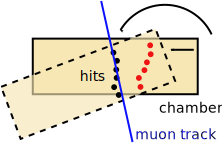
\includegraphics[width=\linewidth]{track_based_alignment.pdf}

\column{0.6\linewidth}
\begin{itemize}
\item Find corrections to assumed chamber positions by minimizing residuals \mbox{(track intersection $-$ hit position)}
\end{itemize}
\end{columns}

\vfill
\begin{columns}
\column{0.5\linewidth}
\begin{itemize}
\item Muon chambers are internally well aligned: 6 degree-of- freedom rigid bodies
\item Combine internal hits into 4-component residuals:
\begin{itemize}\setlength{\itemsep}{0.2 cm}
\item $x$, $y$ position residuals
\item $\tan^{-1} \big(\frac{dx}{dz}\big)$, $\tan^{-1} \big(\frac{dy}{dz}\big)$ angle residuals
\end{itemize}
\item \mbox{Alignment corrections influence multiple residuals components with\hspace{-10 cm}} \\ \mbox{different dependencies on track position, entrance angle: a highly\hspace{-10 cm}} \\ \mbox{constrained system of equations\hspace{-10 cm}}
\end{itemize}

\column{0.5\linewidth}
\vspace{-1 cm}
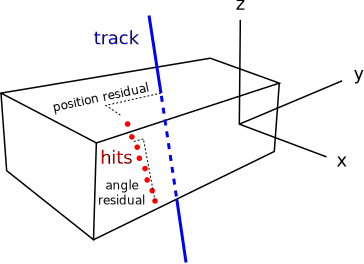
\includegraphics[width=\linewidth]{coordinates.pdf}

\vspace{1 cm}
\end{columns}
\end{frame}

\begin{frame}
\frametitle{Global alignment of the CMS tracking system}

\begin{itemize}
\item Inner silicon tracker and muon chambers must be aligned in the same coordinate system
\begin{enumerate}\setlength{\itemsep}{0.2 cm}
\item Align the tracker independently

\vspace{0.05 cm}
\begin{itemize}\setlength{\itemsep}{0.1 cm}
\item homogeneous magnetic field, low-material environment
\item resolve chicken-and-egg problem of track-fitting and detector
  component alignment with three methods: iteration/convergence,
  simultaneous solution in a large matrix, accumulate knowledge of
  systematic effect in track-fitter
\end{itemize}

\item Fit tracks with aligned tracker, propagate into muon system

\item Align muon chambers with the fixed tracks

\vspace{0.1 cm}
\begin{itemize}\setlength{\itemsep}{0.1 cm}
\item propagates alignment knowledge from high-precision tracker to the rest of CMS
\item automatically resolves chicken-and-egg problem: track-fits and alignment are independent
\item scattering in iron statistically broadens distributions, but does not introduce systematic bias
\end{itemize}
\end{enumerate}
\end{itemize}
\end{frame}

\begin{frame}
\frametitle{Alignment before first collisions}

\mbox{\hspace{-1 cm}
\begin{tabular}{c c}
\includegraphics[height=4 cm]{cosmics.pdf} & \includegraphics[height=4 cm]{beamhalo.pdf} \\
Cosmic rays for barrel & LHC ``beam-halo'' for endcaps
\end{tabular}}

\vspace{0.5 cm}
\hspace{-0.83 cm} \textcolor{darkblue}{\large Cosmic ray and beam-halo alignments provide}

\begin{itemize}
\item a test of the alignment techniques in a fully realistic environment
\item improved momentum resolution for ongoing cosmic ray analyses
\item a future cross-check using non-projective tracks
\begin{itemize}
\item non-projective tracks relate alignable detector elements in different combinations than interaction point muons
\end{itemize}
\end{itemize}
\end{frame}

\begin{frame}
\frametitle{Beam-halo alignment method}

\vspace{-0.15 cm}
\begin{columns}
\column{0.75\linewidth}
\vspace{0.3 cm}
\begin{itemize}
\item Endcap muon chambers were designed with a small overlap region for alignment
\item Tracks passing through overlap region connect chambers without
  any intervening scattering material or long-distance propagation
\item \textcolor{darkblue}{High-precision relative pair-wise alignment}
\item Propagate around each ring with a simultaneous solution of 18 (36) chambers $\times$ 3 parameters \mbox{(1 translation, 2 angles)\hspace{-5 cm}}
\end{itemize}

\column{0.25\linewidth}
\includegraphics[width=\linewidth]{overlaps.png}
\end{columns}

\vspace{0.3 cm}
\textcolor{darkblue}{Simplified example:}

\includegraphics[width=\linewidth]{matrix_description_onestation.png}
\end{frame}

\begin{frame}
\frametitle{Test of the method in Monte Carlo}

\begin{itemize}
\item Procedure applied to Monte Carlo sample with statistics comparable to 2008 LHC single-beam run
\item Predict accuracy by comparing value of each parameter for each chamber with MC-truth
\end{itemize}

\vfill
\includegraphics[width=0.33\linewidth]{mc_rphi.png}
\includegraphics[width=0.33\linewidth]{mc_phiz.png}
\includegraphics[width=0.33\linewidth]{mc_phiy.png}

\end{frame}

\begin{frame}
\frametitle{Results from 2008 LHC single-beam run}

\vspace{0.2 cm}
\mbox{\hspace{-0.45 cm}
\begin{minipage}{\linewidth}
\begin{itemize}
\item Real-data track-based alignment \textcolor{darkblue}{independently verified} by \\ photogrammetry (alignment from a literal photograph of \mbox{the detector)\hspace{-1 cm}}
\end{itemize}
\end{minipage}}

\begin{columns}
\column{0.25\linewidth}
\vspace{-1 cm}
\begin{itemize}
\item Both saw corrections relative to the design description, with high correlation
\end{itemize}

\column{0.75\linewidth}
\hfill \includegraphics[width=0.95\linewidth]{data_correlations.png}
\end{columns}

\begin{columns}
\column{0.4\linewidth}
\includegraphics[width=\linewidth]{residuals_just_before_and_after.png}

\column{0.6\linewidth}
\begin{itemize}
\item Application of track-based alignment narrows and centers residuals distribution, improves tracks
\end{itemize}
\end{columns}
\end{frame}

\begin{frame}
\frametitle{Results from 2008 LHC single-beam run}

\vspace{0.2 cm}
\mbox{\hspace{-0.5 cm}\begin{minipage}{\linewidth}
\begin{itemize}
\item Chamber-by-chamber comparisons with photogrammetry:
\begin{itemize}\setlength{\itemsep}{0.1 cm}
\item agreement with \textcolor{darkblue}{270~$\mu$m} position and \textcolor{darkblue}{0.35~mrad} \mbox{angular accuracy\hspace{-1 cm}}
\item close to the 166~$\mu$m intrinsic hit uncertainty \mbox{(for these chambers)\hspace{-1 cm}}
\item from 33,000 events: \textcolor{darkblue}{9 minutes} of LHC beam \mbox{(3/4 of the 2008 run)\hspace{-2 cm}}
\end{itemize}
\end{itemize}
\end{minipage}}

\vspace{0.4 cm}
\includegraphics[width=0.5\linewidth]{data_rphi.png}
\includegraphics[width=0.5\linewidth]{data_phiz.png}
\end{frame}

\end{document}
